% Flow-PPO experiment analysis: collapse diagnosis + next-step plan.
% Compile: pdflatex experiment_analysis.tex (run twice for toc / refs / hyperref).
% Requires: graphicx, tikz, booktabs, amsmath, enumitem, xcolor, hyperref, caption.
\documentclass[11pt]{article}

\usepackage[utf8]{inputenc}
\usepackage[T1]{fontenc}
\usepackage{lmodern}
\usepackage[a4paper,margin=1in]{geometry}
\usepackage{amsmath,amssymb,bm}
\usepackage{booktabs}
\usepackage{array}
\usepackage{enumitem}
\usepackage{caption}
\usepackage{graphicx}
\usepackage{xcolor}
\usepackage{tikz}
\usetikzlibrary{arrows.meta,positioning,calc}
\usepackage[colorlinks=true,linkcolor=blue,citecolor=blue,urlcolor=teal]{hyperref}

\graphicspath{{figures/}}

% Absorb long \code{} paths / tokens at line ends without overfull boxes.
\emergencystretch=3em

\tikzset{
  phase/.style={draw, rounded corners, align=left, text width=12.6cm, fill=blue!5,
                font=\small, inner sep=6pt},
  flow/.style={-{Stealth[length=2.6mm]}, very thick},
}

\newcommand{\code}[1]{\texttt{#1}}

\title{\textbf{Flow-PPO Experiment Analysis}\\[2pt]
\large Why Every Run Collapses, and What to Fix First}
\author{Flow-Factory}
\date{\today}

\begin{document}
\maketitle

\begin{abstract}
Source: W\&B project \code{Flow-PPO} (entity
\code{315229706-xi-an-jiaotong-university-}), 15 runs across 6 commits, SD3.5-Medium
LoRA $+$ PickScore. Data was pulled and plotted with the repository \code{.venv}; raw
dumps live under \code{.scratch/ppo\_wandb/}. This note diagnoses a failure mode common
to \emph{every} configuration tried so far---a fast rise to a reward ceiling followed by
a slow collapse---identifies its mechanism (reward over-optimization with no KL anchor,
plus a critic that barely beats a mean baseline), and proposes a phased experiment plan
that fixes most variables and solves the collapse first.
\end{abstract}

\section*{TL;DR}
\begin{enumerate}[leftmargin=1.5em]
  \item \textbf{Every configuration shows the same curve}: a fast rise to an
  eval-PickScore ceiling of ${\sim}0.83$--$0.84$ (from the $0.769$ base), then a slow
  monotone collapse. No config sustains gains; the longer a run trains, the more it gives
  back (Fig.~\ref{fig:collapse}, Fig.~\ref{fig:peak}).
  \item \textbf{The collapse is reward over-optimization (reward hacking / distribution
  drift), not numerical instability.} The PPO ratio sits at ${\sim}1.0$ and policy
  grad-norm at ${\sim}3\mathrm{e}{-4}$ throughout---no blow-up, just a tiny, persistent,
  \emph{uncorrected} push toward the reward model. Crucially, \code{kl\_beta = 0} in
  \emph{every} run: the one regularizer that prevents this was never enabled
  (Fig.~\ref{fig:trainlong}).
  \item \textbf{The value critic barely earns its keep.} For the standalone critic,
  explained variance ${\approx}0$---it just predicts the running mean reward, so PPO
  degenerates into REINFORCE-with-a-mean-baseline. The \textbf{backbone critic
  (Scheme~B)} is measurably better (explained variance ${\to}0.2$); the
  \textbf{single-SDE bandit critic} is worse (negative explained variance)
  (Fig.~\ref{fig:explvar}).
  \item \textbf{Recommendation:} stop sweeping warmup / re-warmup / critic-follow knobs.
  Fix everything to one simple baseline and solve the collapse first with a KL anchor $+$
  an early-stop metric. Only then optimize the critic body. See \S\ref{sec:reco}.
\end{enumerate}

\tableofcontents

\section{What was run (config matrix)}
\label{sec:matrix}

All runs are SD3.5-Medium, LoRA, PickScore reward, $10$ inference steps (except two
$40$-step backbone runs), \code{group\_size}~$1$. The axes that actually vary:
\begin{itemize}[leftmargin=1.5em,itemsep=1pt]
  \item \textbf{Warmup}: \code{critic\_warmup\_steps} (warm); periodic re-warmup
  \code{critic\_warmup\_interval} (rwI) / \code{critic\_rewarmup\_steps} (rwS).
  \item \textbf{Critic-follows-policy}: \code{update\_critic\_in\_optimize} (updC) ---
  True $=$ critic trained jointly each optimize step; False $=$ critic only via
  warmup/re-warmup bursts.
  \item \textbf{Value-net structure}: \code{critic\_type} --- \code{standalone}
  (lightweight PMA net) vs \code{backbone} (Scheme~B: diffusion backbone $+$ value head,
  the ``Explicit Critic'' direction) vs \code{backbone\_branches}.
  \item \textbf{Algorithm}: \code{sde\_step\_selection} --- \code{global} (full-SDE PPO)
  vs \code{per\_sample} (single-step SDE / bandit).
  \item Older \code{4bdec9d2} runs predate the \code{critic\_type} /
  \code{sde\_step\_selection} fields; they are the implicit standalone $+$ global path.
\end{itemize}

\begin{table}[h]
\centering
\caption{Configuration matrix (sorted by run length). ``--'' $=$ field absent at that commit.}
\label{tab:matrix}
\resizebox{\textwidth}{!}{%
\begin{tabular}{l l l c c c c l c c c}
\toprule
\textbf{run} & \textbf{commit} & \textbf{critic} & \textbf{warm} & \textbf{rwI} & \textbf{rwS} & \textbf{updC} & \textbf{sde\_sel} & \textbf{infer} & \textbf{kl\_beta} & \textbf{gscale} \\
\midrule
rewarmup-10-6                 & 87dc126c & standalone & 30 & 10  & 6  & False & global     & 10 & 0 & 1   \\
default-cfg                   & 87dc126c & standalone & 30 & 0   & 0  & True  & global     & 10 & 0 & 4.5 \\
rewarmup-10-6\_update-critic  & 87dc126c & standalone & 30 & 10  & 6  & True  & global     & 10 & 0 & 1   \\
sd3-5\_..\_512\_q1\_warm50    & 4bdec9d2 & standalone & 50 & --  & -- & --    & global     & 10 & 0 & 1   \\
default-standalone            & 9c54d8f0 & standalone & 30 & 0   & 0  & True  & global     & 10 & 0 & 1   \\
sd3-5\_..\_256\_q1            & 4bdec9d2 & standalone & 30 & --  & -- & --    & global     & 10 & 0 & 1   \\
backbone ($\times 2$)         & d0482331 & backbone   & 30 & 0   & 0  & True  & global     & 10 & 0 & 1   \\
sd3-5\_..\_512\_q1            & 4bdec9d2 & standalone & 30 & --  & -- & --    & global     & 10 & 0 & 1   \\
single-sde                    & 9b032788 & standalone & 30 & 0   & 0  & True  & per\_sample& 10 & 0 & 1   \\
sd3-5\_..\_rewarmup-100-10    & 9b032788 & standalone & 30 & 100 & 10 & False & global     & 10 & 0 & 1   \\
rewarmup-10-5                 & 87dc126c & standalone & 30 & 10  & 5  & False & global     & 10 & 0 & 1   \\
sd3-5\_..\_512\_q4            & 4bdec9d2 & standalone & 30 & --  & -- & --    & global     & 10 & 0 & 1   \\
explicit\_critic              & 81511ef7 & backbone\_branches & 15 & 0 & 0 & True & global & 40 & 0 & 1   \\
backbone\_infer40             & 81511ef7 & backbone   & 30 & 0   & 0  & True  & global     & 40 & 0 & 1   \\
\bottomrule
\end{tabular}%
}
\end{table}

\paragraph{Commit legend.}
\code{4bdec9d2} initial critic PPO (value net $+$ GAE);
\code{9b032788} group\_size$=$1, samples$=$128;
\code{87dc126c} project rename (after multi-axis logging);
\code{d0482331} add backbone critic (Scheme~B);
\code{9c54d8f0} backbone-critic LoRA align;
\code{81511ef7} dedup / collapse PPO critic-mode branches.

\paragraph{The design-space explosion is real.}
The axes multiply out to warmup $\{30,50,15\}$, re-warmup $\{$off$,10/5,10/6,100/10\}$,
updC $\{$T$,$F$\}$, critic $\{$standalone, backbone, branches$\}$, algo $\{$global,
per\_sample$\}$, and infer $\{10,40\}$. With 15 runs this grid is far from covered, and
\textbf{the one variable theory says matters most (\code{kl\_beta}) is fixed at $0$
everywhere.}

\section{Finding 1 --- Universal rise-then-collapse}
\label{sec:f1}

\begin{figure}[h]
\centering
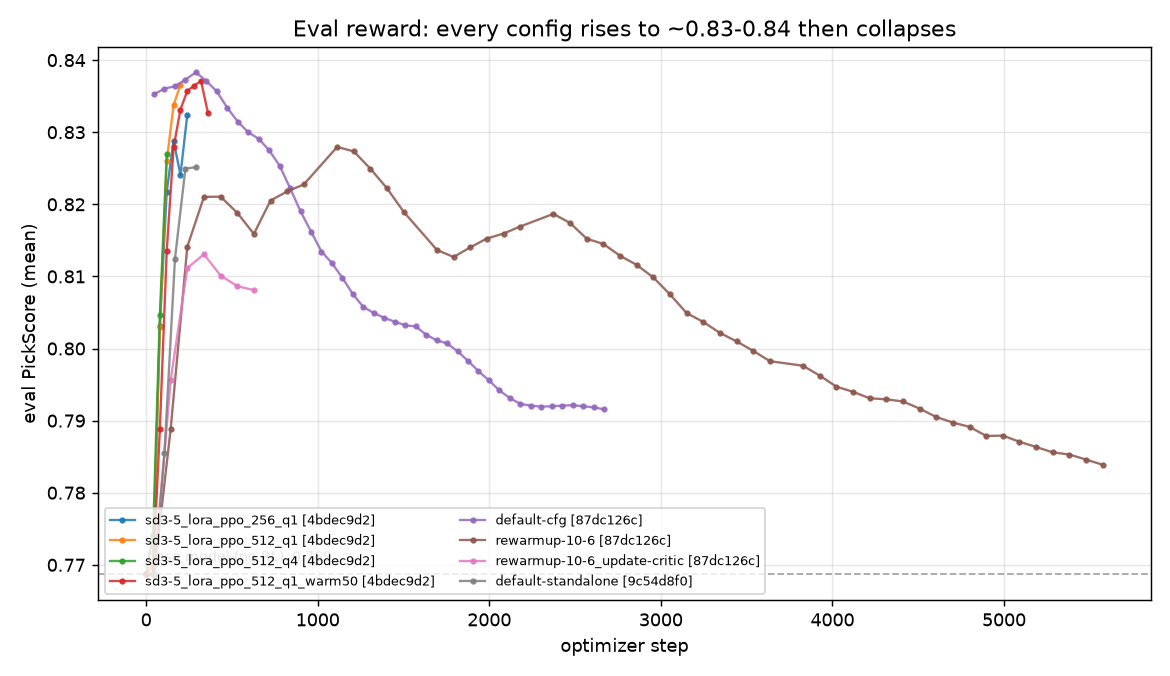
\includegraphics[width=\textwidth]{fig1_eval_reward_collapse.png}
\caption{Eval PickScore vs.\ optimizer step. Every run rises from the $0.769$ base to
${\sim}0.83$--$0.84$, then declines. The two long runs (\code{default-cfg} purple,
\code{rewarmup-10-6} brown) make the trajectory unambiguous.}
\label{fig:collapse}
\end{figure}

The two long runs make the trajectory clear:
\begin{itemize}[leftmargin=1.5em,itemsep=1pt]
  \item \code{default-cfg} (2728 steps): eval peaks \textbf{0.838 @ step 290}, decays to
  \textbf{0.792}.
  \item \code{rewarmup-10-6} (5611 steps, longest): eval peaks \textbf{0.828 @ step
  1113}, decays to \textbf{0.784}; train reward collapses hardest,
  $0.814\!\to\!0.650$.
\end{itemize}
Short runs (${<}400$ steps) look ``fine'' only because they were stopped near the peak;
their train reward is already turning over. There is no qualitative difference between
configs---only ``how long until it rolls over.''

\begin{table}[h]
\centering
\caption{Peak vs.\ final reward (sorted by eval peak). Base model $=0.769$.}
\label{tab:outcome}
\small
\resizebox{\textwidth}{!}{%
\begin{tabular}{l l r r r r r}
\toprule
\textbf{run} & \textbf{commit} & \textbf{max\_step} & \textbf{eval\_peak} & \textbf{eval\_final} & \textbf{train\_peak} & \textbf{train\_final} \\
\midrule
default-cfg                  & 87dc126c & 2728 & 0.838 & 0.792 & 0.836 & 0.752 \\
sd3-5\_..\_512\_q1\_warm50   & 4bdec9d2 & 398  & 0.837 & 0.833 & 0.836 & 0.762 \\
sd3-5\_..\_512\_q1           & 4bdec9d2 & 209  & 0.837 & 0.837 & 0.831 & 0.819 \\
sd3-5\_..\_256\_q1           & 4bdec9d2 & 243  & 0.832 & 0.832 & 0.830 & 0.828 \\
rewarmup-10-6                & 87dc126c & 5611 & 0.828 & 0.784 & 0.814 & 0.650 \\
sd3-5\_..\_512\_q4           & 4bdec9d2 & 131  & 0.827 & 0.827 & 0.836 & 0.808 \\
default-standalone           & 9c54d8f0 & 350  & 0.825 & 0.825 & 0.827 & 0.782 \\
rewarmup-10-6\_update-critic & 87dc126c & 706  & 0.813 & 0.808 & 0.816 & 0.767 \\
backbone                     & d0482331 & 227  & --    & --    & 0.825 & 0.808 \\
single-sde                   & 9b032788 & 188  & --    & --    & 0.777 & 0.741 \\
explicit\_critic             & 81511ef7 & 106  & --    & --    & 0.786 & 0.777 \\
\bottomrule
\end{tabular}%
}
\end{table}

\begin{figure}[h]
\centering
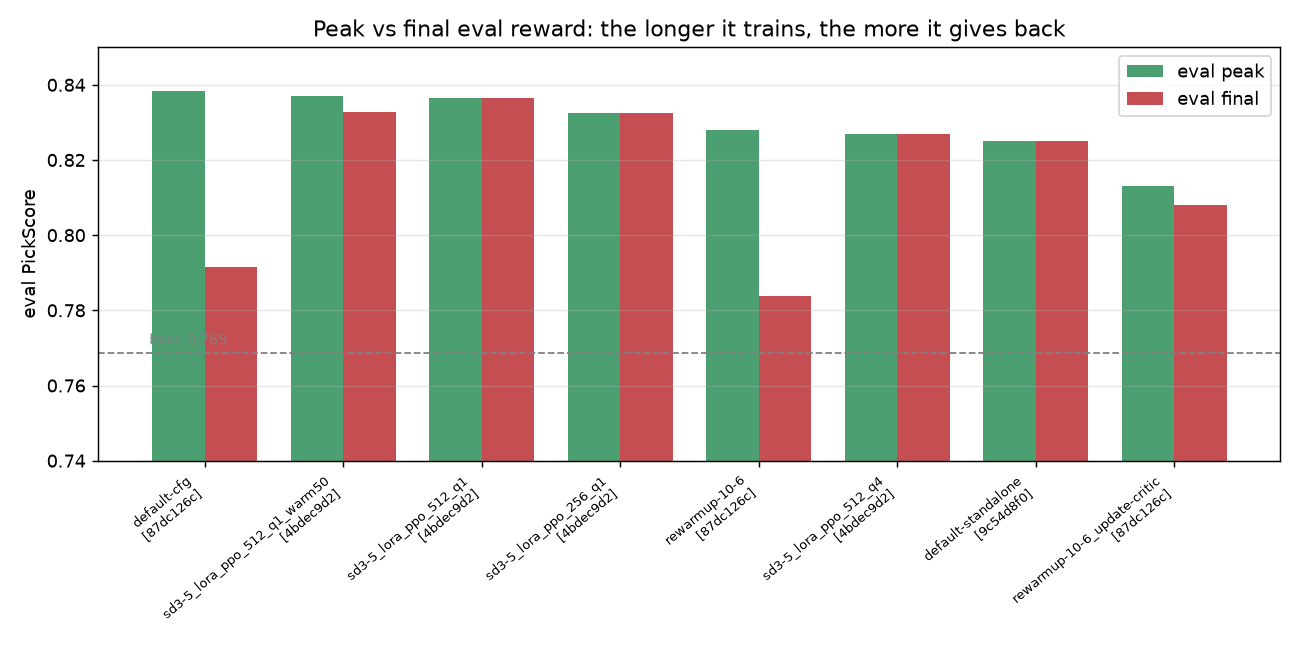
\includegraphics[width=0.95\textwidth]{fig4_peak_vs_final.png}
\caption{Peak vs.\ final eval reward per config. The longer it trains, the more of the
peak it gives back; short runs merely stopped near the top.}
\label{fig:peak}
\end{figure}

\section{Finding 2 --- The collapse is over-optimization, not instability}
\label{sec:f2}

\begin{figure}[h]
\centering
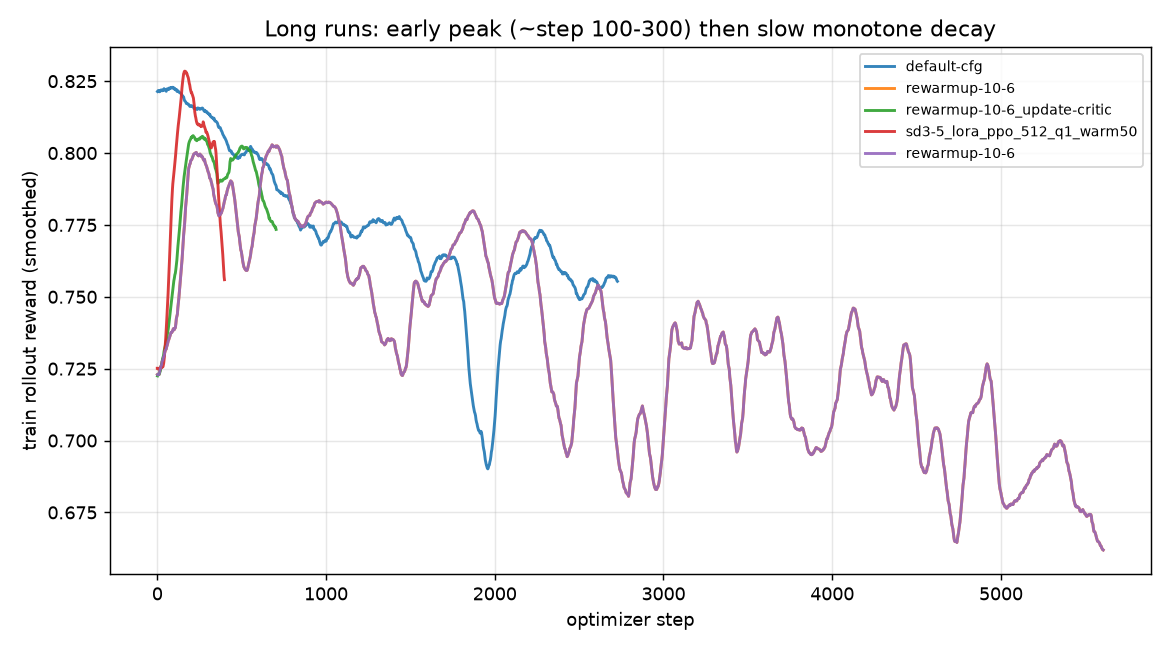
\includegraphics[width=\textwidth]{fig2_train_reward_longruns.png}
\caption{Smoothed train rollout reward for the long runs: an early peak (step
${\sim}100$--$300$) then slow monotone decay over thousands of steps.}
\label{fig:trainlong}
\end{figure}

Windowed diagnostics for the long runs (means per ${\sim}1/6$ of training):

\begin{table}[h]
\centering
\small
\begin{tabular}{l r r r r r r}
\toprule
\textbf{run} & \textbf{step} & \textbf{eval} & \textbf{train\_rwd} & \textbf{expl\_var} & \textbf{ratio} & \textbf{grad\_norm} \\
\midrule
default-cfg   & ${\sim}226$  & 0.837 & 0.815 & $-0.05$ & 1.0000 & $8\mathrm{e}{-4}$ \\
default-cfg   & ${\sim}1137$ & 0.810 & 0.774 & $0.03$  & 1.0000 & $6\mathrm{e}{-4}$ \\
default-cfg   & ${\sim}2500$ & 0.792 & 0.758 & $0.02$  & 1.0000 & $5\mathrm{e}{-4}$ \\
rewarmup-10-6 & ${\sim}465$  & 0.811 & 0.778 & $-0.01$ & 1.0000 & $5\mathrm{e}{-4}$ \\
rewarmup-10-6 & ${\sim}5143$ & 0.787 & 0.688 & $0.02$  & 1.0000 & $6\mathrm{e}{-4}$ \\
\bottomrule
\end{tabular}
\end{table}

The mechanism is clear:
\begin{itemize}[leftmargin=1.5em]
  \item \textbf{\code{ratio}${\approx}1.0000$ and \code{grad\_norm}${\approx}5\mathrm{e}{-4}$
  throughout.} With the tiny flow clip (\code{clip\_range}${=}\pm10^{-4}$) and
  per-dimension-averaged Gaussian log-probs, each PPO step moves the policy a hair.
  \emph{Nothing explodes}---so the collapse is not LR/clip instability but the slow
  accumulation of a \emph{consistently biased} direction.
  \item \textbf{That biased direction is ``maximize PickScore with no anchor.''}
  \code{kl\_beta}${=}0$, so nothing pulls the policy back toward the base model. This is
  the textbook RLHF over-optimization curve: proxy reward and even the eval metric rise,
  peak, then the policy walks off the manifold the reward model was trained on and the
  score decays. Eval peaks (step ${\sim}290$--$1113$) \emph{before} train reward fully
  turns over---a hallmark of reward hacking rather than learning.
\end{itemize}

\noindent\textbf{Implication.} Every knob swept so far (warmup length, re-warmup cadence,
critic-follow) is downstream of the real problem. None addresses the missing anchor, so
none stops the collapse---and \code{rewarmup-10-6} (the most aggressive re-warmup) ran
longest and collapsed \emph{hardest}.

\section{Finding 3 --- The critic barely earns its keep}
\label{sec:f3}

\begin{figure}[h]
\centering
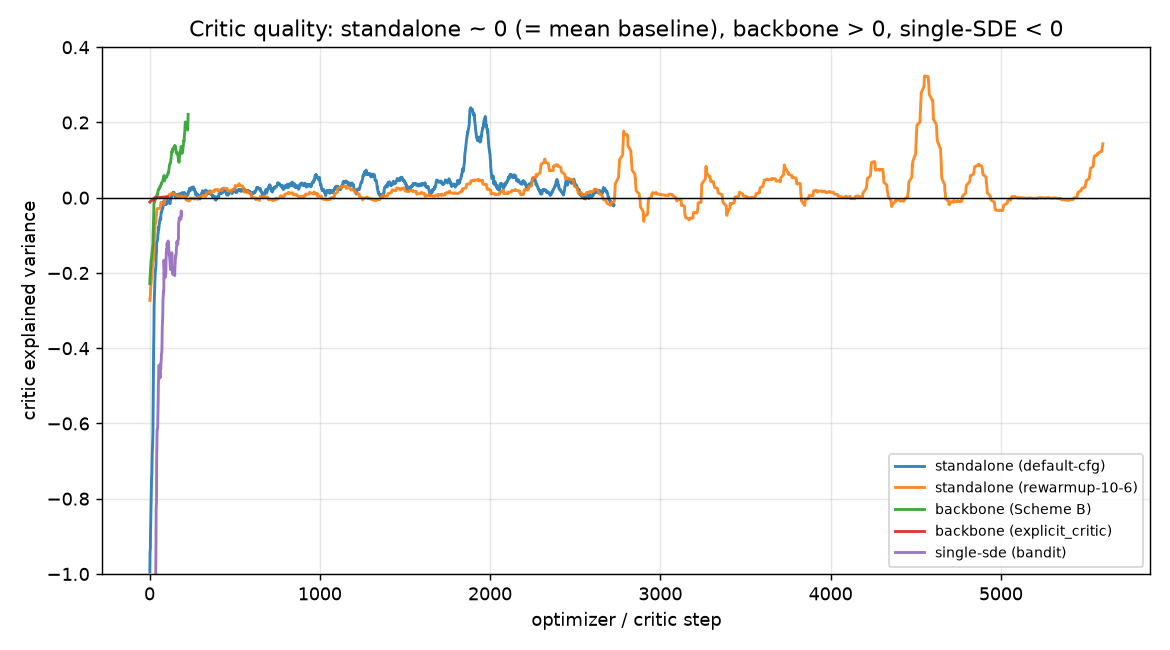
\includegraphics[width=\textwidth]{fig3_critic_explained_variance.png}
\caption{Critic explained variance ($1=$ perfect, $0=$ no better than the mean, $<0=$
worse than the mean). Standalone hovers at $0$; backbone (Scheme~B) climbs to
${\sim}0.2$; single-SDE is negative.}
\label{fig:explvar}
\end{figure}

\begin{itemize}[leftmargin=1.5em]
  \item \textbf{Standalone critic ${\approx}0$.} Because PickScore variance is tiny,
  \code{value\_loss} looks ``good'' (${\sim}0.001$) but that is an illusion: the critic
  just tracks the running \emph{mean} reward (\code{value\_mean}${\approx}$\code{train\_reward}
  in every window). So \code{advantage}${=}R-V\approx R-\mathrm{mean}(R)$---PPO here is
  effectively \textbf{REINFORCE with a mean baseline}, buying nothing over a GRPO-style
  baseline.
  \item \textbf{Backbone critic (Scheme~B) is the only critic with signal}---explained
  variance climbs to ${\sim}0.1$--$0.2$ within $200$ steps. This matches the
  Explicit-Critic-Guidance thesis (a state-aligned backbone value head is a genuinely
  better critic) and is the most promising structural lead, but every backbone run so far
  is ${\le}227$ steps---\emph{unproven past the peak}.
  \item \textbf{Single-SDE (bandit) critic is negative} (down to $-0.5\ldots-5$ early,
  settling slightly below $0$). With one stochastic step the per-state value target is
  high-variance and the critic ends up \emph{worse} than a constant. That run also had
  the weakest reward (train $0.78$) and still collapsed. \textbf{Single-SDE is not the
  place to debug right now.}
\end{itemize}

\section{Per-axis read}
\label{sec:peraxis}

\begin{table}[h]
\centering
\caption{What the data says about each knob.}
\label{tab:peraxis}
\small
\begin{tabular}{p{3.0cm} p{3.6cm} p{7.0cm}}
\toprule
\textbf{Axis} & \textbf{Variants tried} & \textbf{Verdict from data} \\
\midrule
KL anchor \code{kl\_beta} & only \textbf{0} (all runs) & \textbf{Untested and almost certainly the root cause.} Highest-priority variable. \\
Warmup steps & 15, 30, 50 & No effect on collapse; warm50 peaked the same and rolled over. \\
Periodic re-warmup & off, 10/5, 10/6, 100/10 & Does \emph{not} prevent collapse; \code{rewarmup-10-6} ran longest and collapsed hardest. Complexity for no benefit. \\
Critic-follows-policy \code{updC} & True / False & \code{updC=True} decayed slightly more gently but still no growth; second-order. \\
Value-net structure & standalone / backbone / branches & \textbf{Backbone $>$ standalone} on explained variance --- the one structural win, but unproven long-term. \\
Algorithm & global / per\_sample & Single-SDE underperforms (negative expl.\ var, weakest reward). Defer. \\
\code{guidance\_scale} & 1.0 / 4.5 & 4.5 reached the highest peak (0.838) but collapsed like the rest; not a fix. \\
infer steps & 10 / 40 & Backbone-40 too short to conclude. \\
\bottomrule
\end{tabular}
\end{table}

\section{Recommendation --- fix variables, solve collapse first}
\label{sec:reco}

The core problem: ${\sim}6$ axes are co-varied while the single most important one
(\code{kl\_beta}) is pinned at $0$ and the success metric (sustained eval reward) is not
what is being optimized. Change one thing per phase; hold the rest frozen.

\paragraph{Variables to FREEZE (the debug baseline).}
\begin{itemize}[leftmargin=1.5em,itemsep=1pt]
  \item \textbf{Algorithm}: \code{sde\_step\_selection = global} (standard full-SDE PPO);
  drop single-SDE until a baseline works.
  \item \textbf{Warmup}: \code{critic\_warmup\_steps = 30}, \textbf{no periodic re-warmup}
  (\code{critic\_warmup\_interval = 0}), \code{update\_critic\_in\_optimize = True}.
  \item \textbf{Critic structure}: pick ONE; recommended \code{standalone}-512 as the
  cheap control for Phase~1 (so the anchor effect is isolated), backbone held for
  Phase~2.
  \item \textbf{Sampling}: \code{guidance\_scale = 1.0}, \code{group\_size = 1},
  \code{num\_inference\_steps = 10}, current LRs.
  \item \textbf{Success metric}: \textbf{sustained \code{eval/default/reward\_pick\_score\_mean}}
  over a long horizon (e.g.\ ${\ge}1500$ steps), \emph{not} train reward and \emph{not}
  the transient peak.
\end{itemize}

\begin{figure}[h]
\centering
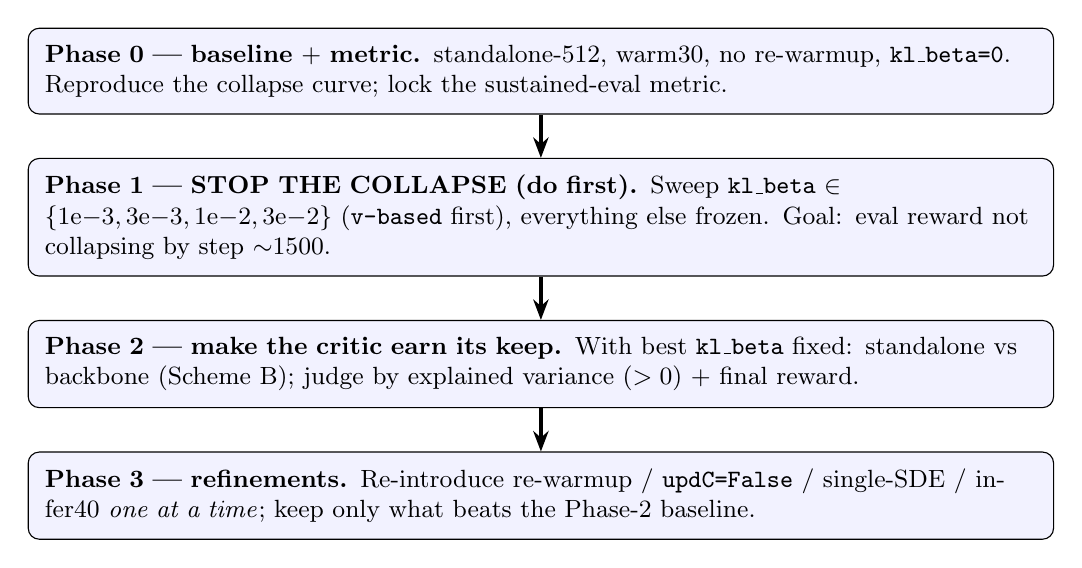
\begin{tikzpicture}[node distance=0.55cm]
  \node[phase] (p0) {\textbf{Phase 0 --- baseline $+$ metric.} standalone-512, warm30, no
    re-warmup, \code{kl\_beta=0}. Reproduce the collapse curve; lock the sustained-eval metric.};
  \node[phase, below=of p0] (p1) {\textbf{Phase 1 --- STOP THE COLLAPSE (do first).} Sweep
    \code{kl\_beta} $\in\{1\mathrm{e}{-3},3\mathrm{e}{-3},1\mathrm{e}{-2},3\mathrm{e}{-2}\}$
    (\code{v-based} first), everything else frozen. Goal: eval reward not collapsing by step ${\sim}1500$.};
  \node[phase, below=of p1] (p2) {\textbf{Phase 2 --- make the critic earn its keep.} With
    best \code{kl\_beta} fixed: standalone vs backbone (Scheme~B); judge by explained
    variance ($>0$) $+$ final reward.};
  \node[phase, below=of p2] (p3) {\textbf{Phase 3 --- refinements.} Re-introduce
    re-warmup / \code{updC=False} / single-SDE / infer40 \emph{one at a time}; keep only
    what beats the Phase-2 baseline.};
  \draw[flow] (p0)--(p1); \draw[flow] (p1)--(p2); \draw[flow] (p2)--(p3);
\end{tikzpicture}
\caption{Phased plan: one variable per phase, collapse solved before critic tuning.}
\label{fig:ladder}
\end{figure}

\paragraph{Phase 1 (first): add the KL anchor.}
Sweep \code{kl\_beta} $\in\{1\mathrm{e}{-3},3\mathrm{e}{-3},1\mathrm{e}{-2},3\mathrm{e}{-2}\}$
with \code{kl\_type = v-based} (cheaper; \code{x-based} ${\sim}1\mathrm{e}{-2}$ as a second
arm), everything else at the frozen baseline. Expect a bias--variance band: too small
$\Rightarrow$ still collapses; too large $\Rightarrow$ never rises. ${\sim}4$ runs, one
variable, directly targets the demonstrated failure---and has never been run.

\paragraph{Phase 2: make the critic real (only after Phase 1 holds).}
With the best \code{kl\_beta} fixed, compare \textbf{standalone vs backbone (Scheme~B)},
judged by explained variance (must be clearly $>0$) and final eval reward. Optionally add
the perturbed-state / branch-$K$ critic target (see \code{docs/ppo/ppo\_analysis}
\S``DiffAC-style perturbed-state critic'') to push explained variance higher.

\paragraph{Phase 3: revisit deferred knobs.}
Re-introduce re-warmup, \code{updC=False} alternation, single-SDE, or 40-step inference
one at a time; keep only what beats the Phase-2 baseline on the sustained-eval metric.

\paragraph{Why this order.}
The collapse is \emph{universal and anchor-shaped}, so no critic/warmup tuning can succeed
until the anchor exists (Phase~1). Once the policy is prevented from walking off-manifold,
critic quality (Phase~2) determines whether PPO actually beats GRPO; everything else is a
refinement (Phase~3). Fix the algorithm to \textbf{global full-SDE PPO with a standalone
critic} as the control, and vary \textbf{only \code{kl\_beta}} first.

\section*{Reproduce}
Histories were pulled from W\&B project \code{Flow-PPO} into
\code{.scratch/ppo\_wandb/\{runs\_raw.json, collapse\_stats.json, hist/*.csv\}} with the
repository \code{.venv} (\code{wandb}, \code{matplotlib}, \code{pandas}). Figures were
regenerated from \code{.scratch/ppo\_wandb/hist/*.csv} into \code{docs/ppo/figures/}; raw
per-run data stays under \code{.scratch/} (git-ignored).

\end{document}
